% ICRA 2027 DRAFT -- work in progress, NOT submission-ready.
% Anonymized for double-blind review per ICRA policy: no author names/affiliations,
% no identifying links. Fill in \author{} and Acknowledgments only at camera-ready.
% See ~/.claude/skills/writing-icra-papers/ for the format/anonymization checklist
% this draft follows.
%
% HARDWARE PLACEHOLDER NOTE: Sections/tables/figures marked [HW-PLACEHOLDER] are
% intentionally left open pending a valid real Kinova Gen3 throw (see
% Sec. results-hw). As of this draft, every non-destructive stage (read-only
% state, gripper actuation, full-speed joint-velocity streaming) has been
% validated live on the real arm, and several real ball throws have been
% executed, but none is a usable data point: bring-up found (1) a
% gripper-release command silently dropped while joint speeds stream (fixed)
% and (2) a 12cm-scale release-position error from an unmodeled end-effector
% offset shared by sim and hardware (quantified, not yet corrected). Do not
% fill these with simulated numbers, and do not report the existing throws
% as data -- leave blank until a throw exists through the corrected model.

\documentclass[conference]{IEEEtran}
\usepackage{graphicx}
\usepackage{amsmath}
\usepackage{amssymb}
\usepackage{booktabs}
\usepackage{xcolor}
\usepackage{cite}
\usepackage{textcomp}
\usepackage{url}

\newcommand{\hwtodo}[1]{\textcolor{red}{\textbf{[HW-PLACEHOLDER: #1]}}}
% SIM-TODO: a real ablation/timing job for this claim was launched from this
% same repo and is running in the background as this draft is written; swap
% for real numbers as soon as it completes, do not guess in the meantime.
\newcommand{\simtodo}[1]{\textcolor{orange}{\textbf{[SIM-RUN-PENDING: #1]}}}
% Short in-table placeholder (the full \hwtodo{} wrapper is too wide to
% repeat across table cells without overflowing the column) -- caption
% already marks the table as a placeholder, so cells just need to read
% as visibly not-real-data.
\newcommand{\hwdash}{\textcolor{red}{\textbf{---}}}

\begin{document}

\title{Torque-Feasible Release-Pose Search for Data-Efficient Robotic
Throwing on a Low-Torque Manipulator}

% BLINDED FOR REVIEW -- do not add names/affiliations before submission.
\author{\IEEEauthorblockN{Anonymous Authors}
\IEEEauthorblockA{Submission for IEEE ICRA 2027 -- Double-Anonymous Review}}

\maketitle

\begin{abstract}
Model-based reinforcement learning has been shown to learn accurate,
data-efficient pick-and-throw (PnT) policies with as few as ten real trials
by combining Gaussian-process dynamics learning with particle-based policy
optimization (MC-PILOT~\cite{turcato2025mcpilot}). That work validates the
approach on a Franka Emika Panda using a release configuration that is fixed
analytically ahead of time -- only the aim and a scalar release speed are
learned. We revisit this design while porting the approach to a
lower-torque 7-DOF arm (Kinova Gen3, 9~Nm wrist actuators) for which the
original fixed-pose strategy turns out not to produce a throw at all. We
extend MC-PILOT along three axes: (1) the release configuration itself is
replaced with a direction-constrained search over the reachable release
state under the arm's real torque and joint-velocity limits, validated
across the whole windup-throw-follow-through trajectory rather than at the
release instant alone; (2) a single policy is trained to generalize across a
\emph{continuous} range of target heights, rather than the paper's discrete
per-height re-optimization; and (3) we quantify a drag-regime crossover
showing model-based learning provides a 3--7$\times$ accuracy gain
specifically where an analytical no-drag baseline breaks down, and is
matched or beaten by that baseline when drag is negligible. A reliability
audit of a reproduced baseline result shows that single-seed convergence
claims can substantially overstate reliability; we report every simulation
result across multiple seeds. In simulation, the approach reaches
1.4--2.7~cm mean landing error across four different manipulators, and the
overhead throw designed for the Gen3's torque envelope reaches 3.15~cm mean
error with a measured, honest 0.83~m safe-throw ceiling. Every
non-destructive stage of the release pipeline -- state read-back, gripper
actuation, full-speed joint-velocity streaming -- has been validated live on
a real Gen3, including several real ball throws; bring-up also surfaced two
hardware-specific failure modes invisible to either simulation track, one
fixed (a gripper-release command silently dropped for as long as joint
speeds are streaming) and one quantified but not yet corrected (a 12~cm
release-position error from an unmodeled 0.12~m end-effector offset).
\hwtodo{real Gen3 throw: mean error (cm), hit rate, $N$ targets, reported
once both fixes are in place and a clean release is confirmed}
\end{abstract}

\begin{IEEEkeywords}
Pick-and-throw, model-based reinforcement learning, Gaussian process
regression, manipulator dynamics, extrinsic dexterity
\end{IEEEkeywords}

\section{Introduction}

Pick-and-throw (PnT) is an appealing alternative to pick-and-place for
industrial and warehouse manipulation: by releasing an object in flight and
letting gravity carry it the rest of the way, a manipulator can service
targets well outside its own reachable workspace, and can do so faster than
a full place motion allows. Executing a precise throw is difficult
precisely because it requires coordinating a high-speed motion with an
uncertain, mid-motion release: object mass, drag, and release-timing
variability all shift the landing point, and small errors compound at
speed.

MC-PILOT~\cite{turcato2025mcpilot} addresses this with a model-based
reinforcement learning (MBRL) approach: a sparse Gaussian-process (GP) model
of the object's ballistic dynamics is learned from a handful of real
throws, and a policy is optimized against that learned model rather than
against the real system directly, giving the approach its data efficiency
(as few as ten real trials to a performing policy). The published
validation is on a Franka Emika Panda with a \emph{fixed} release
configuration (Eq.~31 of~\cite{turcato2025mcpilot}): only the base yaw
(aim) and a scalar release speed are outputs of the learned policy: the
swing itself is a single hand-designed joint trajectory.

This fixed-pose simplification is reasonable for a Panda, whose wrist
actuators can deliver a near-1.2~m/s release speed even with three of seven
joints frozen. It does not transfer to every manipulator. In particular,
the Kinova Gen3 -- a 7-DOF arm with only 9~Nm wrist torque, common in
research labs precisely because it is collaborative-rated rather than
industrial -- cannot produce a usable throw under the paper's fixed-pose
strategy at all: for a fixed low release posture, achievable range falls
off monotonically with elevation angle, so a distance-scoring search
converges on a near-horizontal ``push'' that places the ball rather than
throwing it. Getting a genuine throw out of this class of arm requires
treating the release configuration itself as something to search, not fix
-- and, once it is searched, requires checking torque and velocity
feasibility across the whole trajectory rather than only at the release
instant, since the windup and the post-release recovery can each violate
limits that the release configuration alone satisfies.

This paper reports that extension, together with three further findings
that came out of reproducing and stress-testing MC-PILOT along the way: a
reliability gap in the originally reported baseline convergence, a
continuous (rather than discrete) height-generalized policy, and a
quantified regime in which model-based learning's advantage over an
analytical baseline appears or disappears. All simulation results are
validated across multiple random seeds and independently re-evaluated
through full rigid-body physics on fresh, previously unseen targets --
never read off the training-time cost curve, which we show can sit near
zero while true landing error is off by 17--28\%.

\textbf{Contributions.}
\begin{enumerate}
\item A torque- and velocity-feasible release-pose search that replaces
MC-PILOT's fixed analytical release configuration, validated across the
full windup, throw, and follow-through trajectory. Ablating whole-
trajectory checking against a release-instant-only check on the Gen3 shows
it rejects 83.4\% of candidates the weaker check would have accepted as
feasible, and that a release-instant-only search would have overstated
safely-recoverable range by 25\% (Sec.~\ref{sec:results-ablation}). This
is what makes a low-torque (9~Nm wrist) arm throwable at all under this
framework, and is shown to transfer cleanly to three further manipulators
without per-arm tuning.
\item A reliability audit of a reproduced MC-PILOT baseline: the originally
reported convergence rate is shown to be single-seed luck (true rate 1--2
of 5 seeds), root-caused to unstratified exploration and an unscaled RBF
lengthscale, and fixed to a verified 5-of-5-seed, 250-throw, 100\%
hit-rate result.
\item A single policy generalizing across a \emph{continuous} target-height
range (vs.\ the original paper's single discrete re-optimization
demonstration), plus generalization across four manipulator platforms.
\item A quantified drag-regime crossover: the paper's analytical no-drag
baseline matches or beats MC-PILOT when drag is negligible, and MC-PILOT
wins by 3--7$\times$ once drag is significant -- characterizing exactly
when the learned model earns its cost.
\item A staged, safety-gated hardware bring-up on a real Kinova Gen3: every
non-destructive stage (state read-back, gripper actuation, full-speed
joint-velocity streaming) validated live at all four rehearsal speed
scales, plus several real ball throws. Bring-up surfaced two failure modes
neither simulation track could have found: a gripper-release command
silently dropped for as long as joint speeds are being streamed (fixed with
an in-stream pause, Sec.~\ref{sec:results-hw}), and a 0.12~m tool offset,
read directly from the gripper's own firmware configuration, that the
release solver -- shared identically between simulation and hardware -- has
always modeled as zero, worth 0.39~m/s (26\% of release speed) and 12.0~cm
of release-position error at the trained release state.
\hwtodo{Real thrown-ball results to be reported here once the offset
correction (Sec.~\ref{sec:results-hw}) is applied and re-verified.}
\end{enumerate}

\textbf{Scope note.} Contributions 1--4 are established in simulation,
validated across multiple seeds and, where noted, multiple manipulators.
Contribution 5 is partial as of this draft: every non-destructive hardware
stage is validated live on a real Gen3, and several real ball throws have
been executed, but no real landing has been measured, because the release
model both sim and hardware share has an identified 12~cm-scale error not
yet corrected (Sec.~\ref{sec:results-hw}) -- stated here, at the point a
reader forms expectations for the rest of the paper, rather than left for
Sec.~\ref{sec:results-hw} to disclose.

\section{Related Work}

\textbf{Analytical PnT.} Fully engineered throwing systems
(e.g.\ industrial waste sorting~\cite{turcato2025mcpilot}) achieve high
throughput but require re-engineering whenever the setup changes, since the
trajectory generation is tailored to a specific system model.

\textbf{Model-free PnT.} TossingBot~\cite{zeng2020tossingbot} learns an
end-to-end residual-physics throwing policy purely from outcome data,
requiring hundreds to thousands of trials and testing on a comparatively
small set of fixed target positions; it also fixes the release
\emph{direction} and learns only speed. The motivation, however, is
different from the fixed-pose simplification we revisit here: TossingBot
fixes direction to keep the model-free policy's action space small enough
to learn from real-robot interaction alone, a sample-efficiency
consideration. MC-PILOT's fixed release pose~\cite{turcato2025mcpilot} is
not sample-efficiency-motivated -- its policy optimization runs offline
against a learned model, so a larger action space costs simulated compute,
not real trials -- and was, we infer, simply adequate for a Panda's torque
headroom. The two arrive at superficially similar designs (learn speed,
fix everything else) for unrelated reasons, and only the second reason
breaks down on a lower-torque arm.

\textbf{Constraint-aware trajectory generation.} A substantial body of
work addresses torque- and velocity-constrained trajectory optimization
for manipulators more generally (time-optimal path parameterization,
sampling-based motion planning under dynamics limits, control-barrier-
function and MPC formulations for safety-constrained high-speed motion).
% TODO(lit-review): this paragraph needs specific citations before
% submission -- add 2-4 references for constraint-aware/time-optimal
% trajectory generation and, if any exist, throwing or dynamic-release
% work on collaborative/low-torque arms specifically. Not fabricating
% citations here; flagged for a real literature pass.
Our release-pose search (Sec.~\ref{sec:method-search}) is a search over
discrete posture/direction candidates combined with a per-candidate linear
program and a feasibility cascade, rather than a continuous trajectory
optimizer -- deliberately simpler than general constrained trajectory
optimization, since the object here (a single release state, then two
fixed-shape cubic segments) is much lower-dimensional than a general
motion-planning problem. To our knowledge, no prior PnT work quantifies a
\emph{safe-throw ceiling} (Sec.~\ref{sec:results-overhead}) as a measured
property of a specific low-torque platform, as opposed to assuming
sufficient actuator headroom by choice of robot.

\textbf{Model-based PnT.} MC-PILOT~\cite{turcato2025mcpilot}, building on
the MC-PILCO model-based policy-search framework~\cite{amadio2022mcpilco}
and its own preliminary conference version~\cite{turcato2023codit}, learns
a GP dynamics model plus a release-timing delay distribution and optimizes
a policy against simulated particles drawn from that model. It reaches
near-perfect accuracy on a Panda from ten real trials and demonstrates that
adapting to a new target height requires only re-optimizing the policy
through the already-learned model, without new physical trials. What it
does not address: (i) whether the release configuration itself needs to be
searched, rather than fixed, for arms with less actuator headroom than a
Panda; (ii) whole-trajectory torque/velocity feasibility, as opposed to
release-instant feasibility; (iii) reliability across multiple random
seeds on the real system; and (iv) when, quantitatively, the learned model's
advantage over a closed-form analytical baseline actually holds. These four
gaps are the subject of this paper.

\section{Method}

\subsection{MC-PILOT recap}
Following~\cite{turcato2025mcpilot}, the object's ballistic dynamics are
modeled with three independent sparse GPs (one per Cartesian velocity
component), trained on $(\text{position}, \text{velocity}) \to
\Delta\text{velocity}$ transitions collected from real or simulated
throws. A radial-basis-function (RBF) policy network maps a target position
(and, in our height-generalized variant, a target height) to a release
speed, squashed to $[0, u_M]$. The policy is optimized by propagating
particles through the learned GP model and minimizing expected landing
distance to target, so the entire policy-improvement loop runs offline
against the model between real trials -- the source of the approach's data
efficiency.

\subsection{Release-pose search under real constraints}
\label{sec:method-search}
Where the original work fixes the release joint configuration $q_{rel}$
(Eq.~31 of~\cite{turcato2025mcpilot}) and derives only a base-yaw aim and a
scalar speed, we search the release \emph{state} $(q, \dot q)$ directly.
The search is bilevel: an outer discrete search over release posture $q$
and commanded direction $\hat d$, and an inner linear program that finds
the maximum release speed achievable at that posture/direction under the
arm's real limits.

\textbf{Inner problem (per posture/direction).} For a 7-DOF arm with joint
axes alternating pitch/roll, only the three pitch joints (indices $1,3,5$
in our convention) can contribute velocity perpendicular to a chosen swing
plane; the four roll/twist joints (indices $0,2,4,6$) rotate about axes
that lie roughly along their own links, and allowing the optimizer to use
them produces a corkscrew rather than a throw (verified numerically: with
all roll/twist joints unconstrained, achievable speed collapses toward the
axis where every pitch joint fires in the same rotational sense). We
therefore freeze $\dot q_i = 0$ for $i \in \{0,2,4,6\}$ and solve
\begin{equation}
\begin{aligned}
\max_{\dot q,\, s} \quad & s \\
\text{s.t.} \quad & J(q)\,\dot q = s\,\hat d, \\
& |\dot q_i| \le \dot q_i^{\max} \;\; \forall i, \\
& \dot q_i = 0 \;\; \forall i \in \{0,2,4,6\},
\end{aligned}
\label{eq:release-lp}
\end{equation}
a linear program in $(\dot q, s)$ solved with an interior-point/simplex
solver (\texttt{scipy.optimize.linprog}, HiGHS). The static roll/twist
\emph{angles} (not velocities) remain free search parameters: pinning them
to exactly zero collapses the three pitch axes to parallel, which also
degenerates achievable direction to a single line, so a small static roll
offset is needed to break that degeneracy.

\textbf{Outer problem (posture and direction enumeration).} With the
roll/twist joints' velocities frozen, the reachable release-velocity
directions at a given posture $q$ span a single plane, whose basis we
construct from the cross product of the two free pitch joints' Jacobian
columns. We grid-search the two remaining free pitch angles and the static
roll offset ($5^\circ$ resolution on the two grid axes we sweep most
finely, $8^\circ$ on the third; $\sim\!9\times10^4$ posture combinations
for the Gen3 profile before pruning), and for each posture that clears a
minimum end-effector height and passes static torque feasibility
(gravity-only inverse dynamics against the manufacturer's torque limits),
sweep candidate directions $\hat d$ at elevation angles from $5^\circ$ to
$45^\circ$ (steps of $5^\circ$, both signs) within the posture's swing
plane. Each surviving (posture, direction) pair is scored by
Eq.~\eqref{eq:release-lp} and passed through the feasibility cascade of
Sec.~\ref{sec:method-feasibility}; among all candidates that survive the
full cascade, the one maximizing \emph{true landing distance from the base}
(computed by forward-integrating the drag-augmented ballistic equations
from the candidate's own release position and velocity, not
$\lVert\text{release\_pos}\rVert + \text{flight range}$, which is only
correct when the release point and throw direction are collinear through
the origin) is selected as the release state for this arm.

\textbf{Azimuth propagation.} The single verified release state is
propagated across a full training wedge ($-33^\circ$ to $+33^\circ$ base
azimuth, $3^\circ$ steps) by rotating the base joint angle alone, exploiting
a numerically verified ($10^{-6}$) symmetry: because gravity is
$z$-symmetric, rotating the base by $\Delta$ rotates the whole downstream
Jacobian (and hence every torque/velocity feasibility property already
verified for the seed entry) by the same $\Delta$, exactly. This is
preferred over searching each azimuth independently, which we found
produces large speed discontinuities between adjacent azimuths (an
early, narrower-grid version of this pipeline showed swings from
0.45~m/s to 0.15~m/s across $3^\circ$ of azimuth) that break the runtime
solver's nearest-azimuth interpolation and visibly degrade training
accuracy. A turret-aiming correction accounts for the resulting off-axis
release geometry when a target's true bearing does not match its
table-nearest azimuth entry. The resulting azimuth$\to$pose table is
consumed by one shared solver (\texttt{OptimizedReleaseSolver}) used
identically at training time and at hardware-execution time, so simulation
and hardware plan the same throw by construction; a regression test
asserts the two call sites agree to $10^{-12}$.

\subsection{Whole-trajectory feasibility}
\label{sec:method-feasibility}
An earlier version of this pipeline checked only release-instant torque
feasibility (static gravity torque at the release posture, plus dynamic
torque at the release instant with zero commanded acceleration). This
missed real failure modes discovered only by rendering trajectories and
watching them, then confirmed numerically, motivating a full-trajectory
cascade with four stages, applied in order (a candidate is rejected at the
first stage it fails):

\begin{enumerate}
\item \textbf{Kinematic windup bound.} The windup posture
$q_{windup} = q_{rel} - \dot q_{rel}\,(t_{throw}/2)$ (the start of a
monotonic velocity ramp reaching $\dot q_{rel}$ at release) must lie within
the joint position limits.
\item \textbf{Windup-path torque.} Static torque feasibility only at the
release posture can pass while the neutral$\to$windup swing itself
transits a worse intermediate gravity configuration -- e.g., a shoulder
joint sweeping from a $22^\circ$ neutral to a $90^\circ$ cocked posture can
peak near its torque limit mid-swing even though both endpoints are safe.
We sample 5 points along the straight-line neutral$\to$windup path and
require gravity-only inverse dynamics to stay under 90\% of $\tau_{\max}$
at every sample.
\item \textbf{Throw-ramp torque.} Checking only the release instant
(zero commanded acceleration) misses inertial torque during the ramp
itself, since a cubic velocity profile has nonzero acceleration everywhere
except (generically) one instant; two real training crashes at peak
torque ratios of 1.02 and 1.01 occurred at mid-ramp points this check
does not see. We build the exact cubic windup$\to$release trajectory the
runtime controller uses and sample it at 40 points, evaluating inverse
dynamics plus an explicit Jacobian-transpose feedforward term for the
gripped ball's weight (Sec.~\ref{sec:method-torque}) at every sample,
against 75\% of $\tau_{\max}$.
\item \textbf{Follow-through torque and velocity.} Nothing in the first
three stages constrains the post-release recovery motion. A release
posture that passes all three can still require the arm to decelerate from
an extreme release configuration back to neutral at 1.15--3.2$\times$
$\tau_{\max}$ -- a trajectory that would fault real hardware, and which
looked, on video, like the arm going limp the instant it released the
ball rather than an obviously wrong number. Peak follow-through torque is
not monotonic in recovery duration (it bottoms out and then rises again for
longer durations), so we evaluate 8 candidate recovery durations
(0.6--4.0~s) rather than growing a single guess, sampling 30 points per
duration against both an 85\%-of-$\tau_{\max}$ torque margin \emph{and} the
joint velocity limit (torque alone is insufficient: one duration passed
torque at 95\% of limit while peak velocity sat at 188\% of $\dot
q^{\max}$); a candidate is accepted if \emph{any} of the 8 durations clears
both margins.
\end{enumerate}

Stage 4 (follow-through) is the most expensive per candidate ($8\times30 =
240$ inverse-dynamics evaluations) and, empirically, the stage most likely
to reject a candidate that survives stages 1--3 -- see
Sec.~\ref{sec:results-ablation} for a quantified breakdown.

\subsection{Real, torque-controlled release}
\label{sec:method-torque}
Rather than assigning the ball's release velocity directly
(\texttt{resetBaseVelocity}, the shortcut both the paper's simulated
ablations and an earlier version of this project's own arm-physics track
used), the simulated arm is driven under computed-torque control:
\begin{equation}
\tau = M(q)\,\ddot q_{cmd} + C(q,\dot q) + G(q) + J(q)^\top f_{ball},
\label{eq:computed-torque}
\end{equation}
where the first three terms are the manipulator's own inverse dynamics
(mass matrix, Coriolis/centrifugal, gravity), evaluated by the physics
engine, and $f_{ball} = m_{ball}\,[0,0,g]^\top$ is an explicit
Jacobian-transpose feedforward for the gripped ball's weight. This last
term is necessary because the ball is modeled as a separate rigid body
attached by a grip constraint (needed so it can be released mid-motion by
removing the constraint); the physics engine's own inverse-dynamics call
has no visibility into a body it does not consider part of the kinematic
chain, so without Eq.~\eqref{eq:computed-torque}'s last term the controller
under-compensates for the payload and tracking error grows with commanded
speed. The release velocity used for every reported result is read back
from the physics engine (\texttt{getBaseVelocity}) after the grip
constraint is removed, never assigned -- verified by tracing the code path
for every reported number, not assumed.

Getting this release to match the trained particle model required fixing
three further, independently discovered biases: (i) targets sampled by
distance-and-angle from the \emph{origin}, per the paper's convention,
silently produce unreachable off-axis targets once the release point's
offset from the origin is a non-negligible fraction of the arm's own
range -- fixed by sampling in flight space (an annulus around the actual
release point); (ii) the particle model used for policy optimization
propagated from the \emph{nominal} release position rather than the
\emph{empirical mean} release position actually observed across collected
trials, a several-centimeter systematic bias the velocity-only GP model
cannot learn away since it has no state-position error term; (iii) a
zero-amplitude windup bug, found only by extracting and viewing rendered
frames rather than trusting the reported numbers.

\subsection{Height-generalized policy}
The trajectory-termination plane and the particle-propagation plane in
policy optimization are parameterized by a landing height $h$, and the
policy input is extended to $(P_x, P_y, h)$. We compare (i) a policy
trained and evaluated at a single fixed height, (ii) a policy re-optimized
per discrete height by reusing the trained GP verbatim (reproducing
Sec.~6.4 of~\cite{turcato2025mcpilot}), and (iii) a single policy trained
once over a continuous range of $h$, evaluated at heights never seen during
training.

\section{Experimental Setup}
\label{sec:setup}

\textbf{Simulation.} All arm-physics results use a rigid-body PyBullet
simulation with real manufacturer joint-velocity and torque limits.
Four manipulators are evaluated under the identical pipeline: KUKA iiwa7,
Franka Panda, xArm6, and Kinova Gen3. Targets for the Gen3-specific studies
are sampled in \emph{flight space} -- an annulus around the release point
rather than the origin -- since the release-point offset is a large
fraction of this arm's short reachable range and origin-relative sampling
silently produces unreachable targets.

\textbf{Evaluation protocol.} Training-time particle cost is never reported
as accuracy: every headline number is a re-evaluation through full
rigid-body rollout (\texttt{PyBulletThrowingSystem.rollout}) on fresh,
previously unused RNG seeds and target sets. Multi-seed results use 5
seeds unless noted.

\textbf{Real hardware.} The target platform is a Kinova Gen3 7-DOF arm
(base-plate mounted, 0.433~m above the floor) at a fixed lab bench, driven
via the Kortex SDK over joint-speed streaming
(\texttt{Base.SendJointSpeedsCommand}, single-level servoing, a measured
40~Hz ceiling). Perception uses an Intel RealSense D435i with printed ArUco/ChArUco
targets for camera-to-base extrinsic calibration. Landing measurement
triangulates independently-detected 2D ball centroids from the D435i's
rectified stereo infrared pair, rather than reading its depth map, since
raw D435i depth error (${\sim}2\%$ of range, 2--4~cm at 1--2~m) is
comparable to the landing error being measured and worse still for a
small, low-texture sphere; depth is used only as a coarse detection gate.
A Gauss-Newton fit to pixel reprojection error (not the triangulated 3D
points, whose noise is range-correlated) then solves for the ball's first
floor contact, since a bounced or rolled resting position is a systematic
offset from the quantity the policy's landing error is defined against.

\subsection{Implementation details}
\label{sec:impl-details}
\textbf{Notation.} $q,\dot q \in \mathbb{R}^7$ are joint angle and
velocity; $s$ is release speed and $\hat d$ its commanded unit direction;
$h$ is target/landing height; $u \in [0, u_M]$ is the policy's output
release speed, squashed through $g(x) = \tfrac{u_M}{2}(\tanh(x)+1)$ as
in~\cite{turcato2025mcpilot}; $\tau_{\max}$, $\dot q^{\max}$ are the
per-joint manufacturer torque and velocity limits. These symbols are used
consistently across Secs.~III--V.

\textbf{GP/policy hyperparameters.} The RBF policy lengthscale is
initialized to $0.15\times(l_M - l_m)$, where $[l_m, l_M]$ is the target
distance range, and remains a trained parameter thereafter
(\texttt{flg\_train\_lengthscales=True}) rather than a fixed constant; the
role of the 0.15 factor is only to avoid a dead gradient at initialization
on narrow target domains (Sec.~\ref{sec:results-baseline}), not to encode a
derived optimum. Sparse-GP dynamics models use $M=400$ inducing points,
$N_b=250$ mini-batch size for optimization, matching the real-setup column
of Table~1 in~\cite{turcato2025mcpilot} unless stated otherwise for a
specific ablation.

\textbf{Hardware control/calibration.} The Gen3's joint-speed streaming
interface (\texttt{Base.SendJointSpeedsCommand}, single-level servoing) has
a measured ceiling of 40~Hz; simulation runs physics and control together
at 50~Hz. Camera-to-base extrinsic calibration uses print-ready,
exact-scale ArUco/ChArUco boards with an on-print verification ruler to
catch print-scaling errors before they become calibration errors.

\section{Results}

\subsection{Baseline reliability audit}
\label{sec:results-baseline}
The originally reported baseline result (5/5 hits in 5 trials, single
seed) was re-run across 5 random seeds and converged on only 1--2 of 5
(60\%, 20\%, 80\%, 10\%, 10\% hit rates). The cause was two compounding
issues: unstratified exploration can leave the GP blind to part of the
release-speed range, and an unscaled RBF lengthscale saturates the policy's
output non-linearity so the policy barely varies with target position.
Fixing both (stratified exploration bands, lengthscale initialized to the
target-range scale) restores 5-of-5-seed convergence
(Fig.~\ref{fig:reliability}). A full evaluation with both fixes -- 5 seeds
$\times$ 50 fresh, previously unseen targets, 250 throws total -- reaches
100\% hit rate at both $<$10~cm and $<$5~cm, mean landing error 1.86~cm,
P95 3.17~cm (Fig.~\ref{fig:eval-dist}).

\begin{figure}[t]
\centering
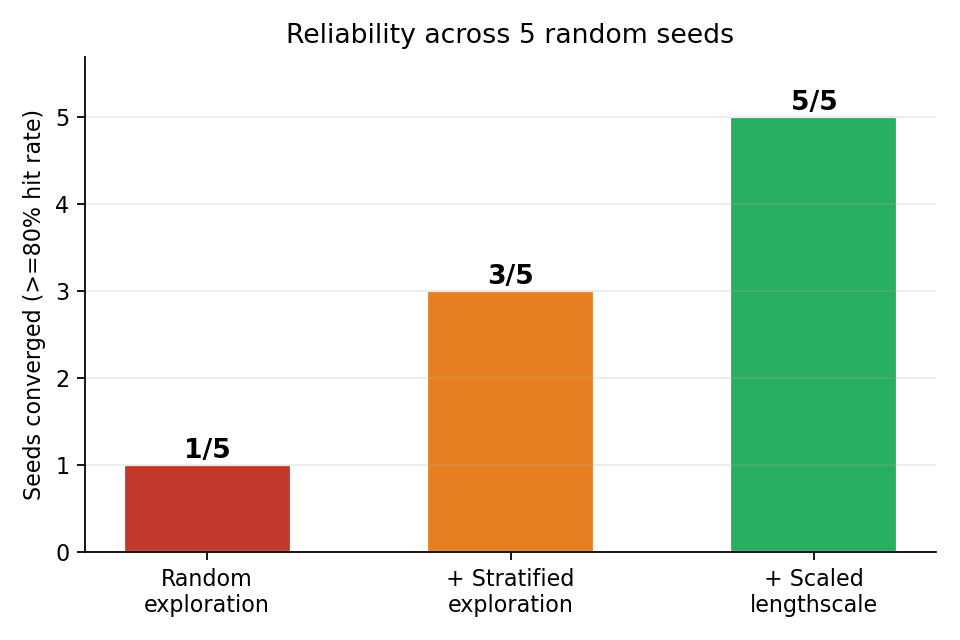
\includegraphics[width=0.9\linewidth]{../status_update/fig2_seeds_converged.png}
\caption{Reliability of the reported baseline result across 5 random seeds,
before and after the exploration/lengthscale fix. The originally reported
single-seed result is not representative of the unfixed configuration.}
\label{fig:reliability}
\end{figure}

\begin{figure}[t]
\centering
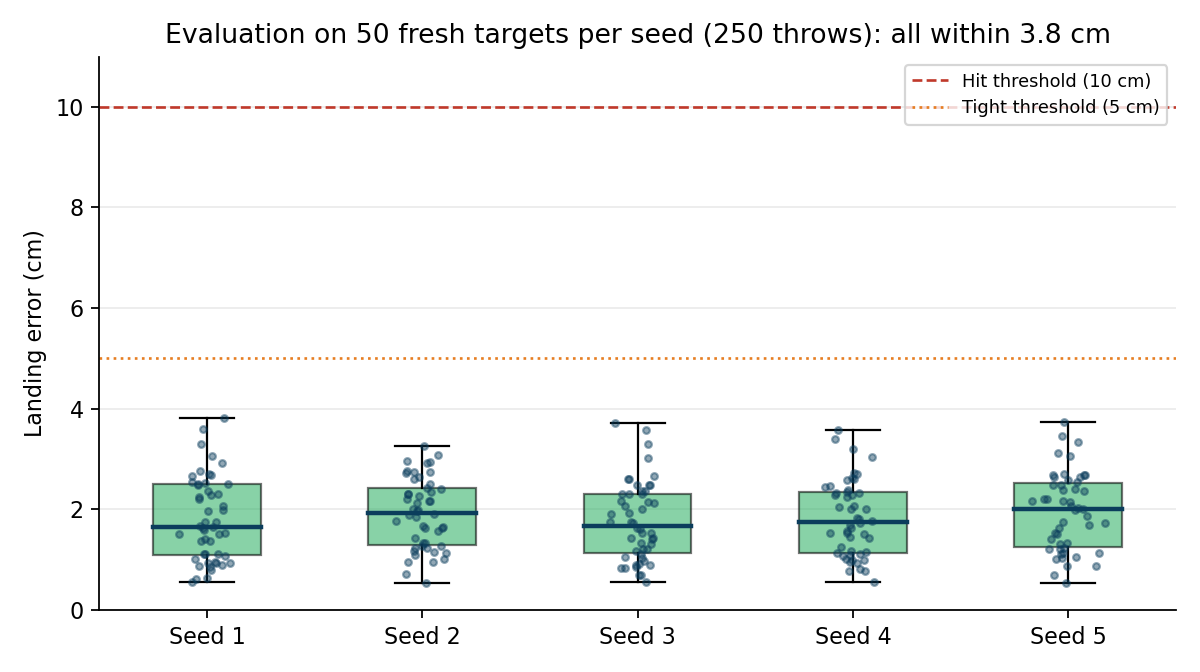
\includegraphics[width=0.9\linewidth]{../status_update/fig6_eval_error_distribution.png}
\caption{Landing-error distribution after the reliability fix: 5 seeds
$\times$ 50 fresh targets, 250 throws, 100\% hit rate at $<$10~cm, mean
error 1.86~cm.}
\label{fig:eval-dist}
\end{figure}

\subsection{Multi-arm generalization and the drag-regime crossover}
\label{sec:results-multiarm}
The release-pose-search pipeline (Sec.~III-B/C) trains cleanly on all four
tested manipulators, reaching 1.4--2.7~cm mean landing error without
per-arm tuning beyond the profile-level torque/velocity limits
(Fig.~\ref{fig:generalization}), confirming the whole-trajectory feasibility
fixes are not specific to the Gen3. Sweeping payload drag from
$<$1\% to $\sim$19\% of gravity and comparing against the paper's
closed-form no-drag analytical release-speed baseline shows a crossover:
at low drag the analytical baseline is already near-optimal and MC-PILOT
adds little, while at high drag the analytical baseline degrades to
4--6~cm error and MC-PILOT holds 0.6--1.7~cm, a 3--7$\times$ gain. Object
generalization at these release speeds (payload mass/size varied without
retraining) is essentially free: landing error stays flat at
$\sim$1.4~cm across 30--150~g and 2--4.5~cm diameters, since drag is
negligible for these objects and the payload feedforward term already
compensates measured mass directly.

\textbf{Why the crossover happens.} The analytical baseline solves the
drag-free ballistic equations, so its landing-distance bias should grow
with the fraction of flight-time deceleration actually contributed by
drag -- to first order, proportional to $C_D \rho A v^2 T / (2m)$, i.e.\
roughly the drag-to-gravity ratio swept in this experiment for the
speed/flight-time regime tested here. The learned GP model instead fits
the \emph{realized} $\Delta v$ directly from data, so its error is set by
the model's own fit quality (inducing-point count, GP noise floor,
particle count) rather than by how large the unmodeled physics term is.
The crossover sits where the analytical model's drag-proportional bias
grows past that roughly constant learned-model error floor. This is a
qualitative scaling argument consistent with the observed crossover, not a
fitted quantitative model -- deriving the exact crossover drag fraction
analytically, and checking it against a finer drag sweep, is future work.

\begin{figure}[t]
\centering
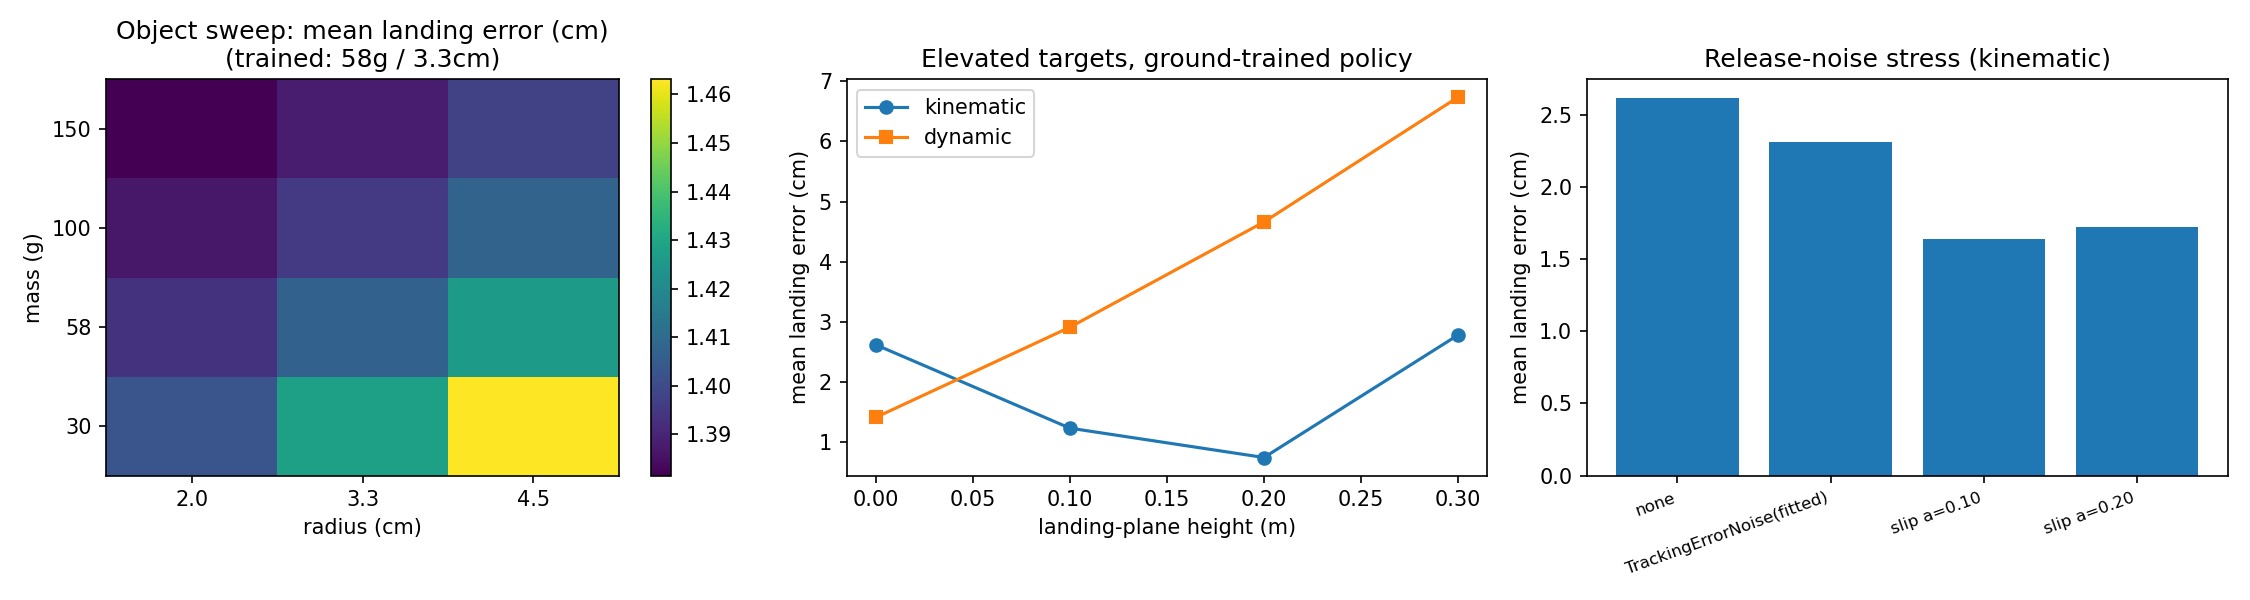
\includegraphics[width=0.9\linewidth]{../mc-pilot-pybullet/results_generalization/generalization.png}
\caption{Landing error across four manipulators (KUKA iiwa7, Franka Panda,
xArm6, Kinova Gen3) under the identical release-pose-search pipeline.}
\label{fig:generalization}
\end{figure}

\subsection{Height generalization}
\label{sec:results-height}
A single policy trained once over a continuous height range and evaluated
on 100 fresh targets at randomly sampled heights never seen during training
reaches 100\% hits, mean error 2.0~cm, worst-case 5.0~cm, with no error
trend against height (Fig.~\ref{fig:height-gen}) -- i.e.\ the policy
generalizes across the range rather than degrading toward its untrained
extremes. Separately, reproducing the original paper's zero-new-trials
height-adaptation claim (Sec.~6.4 of~\cite{turcato2025mcpilot}) on the
real-dynamics overhead throw (Sec.~\ref{sec:results-overhead}) by reusing
the trained GP verbatim and re-optimizing only the policy for three new
heights gives 2.95/3.41/3.80~cm mean error at $h=0.10/0.20/0.30$~m
(Fig.~\ref{fig:height-adapt}), zero additional physical trials per height,
matching or beating both the 3.15~cm ground baseline and a 3.63~cm full
9-D retrain that required a complete new training run.

\begin{figure}[t]
\centering
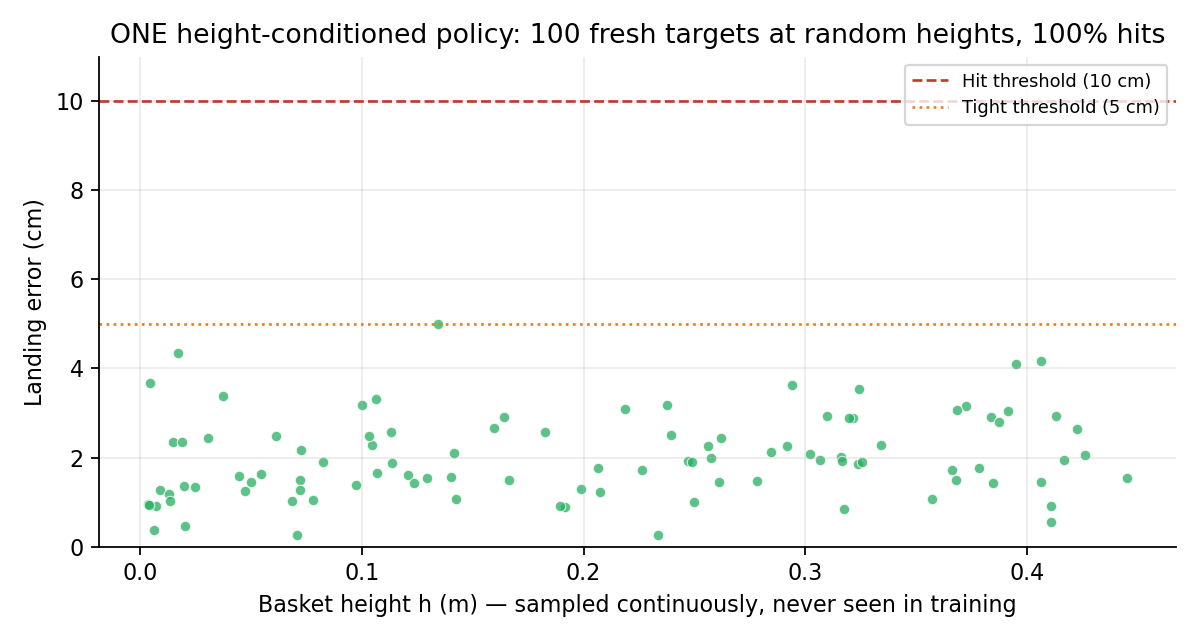
\includegraphics[width=0.9\linewidth]{../status_update/for_prof/fig11_hgen_error_vs_height.png}
\caption{Landing error vs.\ target height for the continuously
height-generalized policy, 100 fresh targets at heights never seen in
training.}
\label{fig:height-gen}
\end{figure}

\begin{figure}[t]
\centering
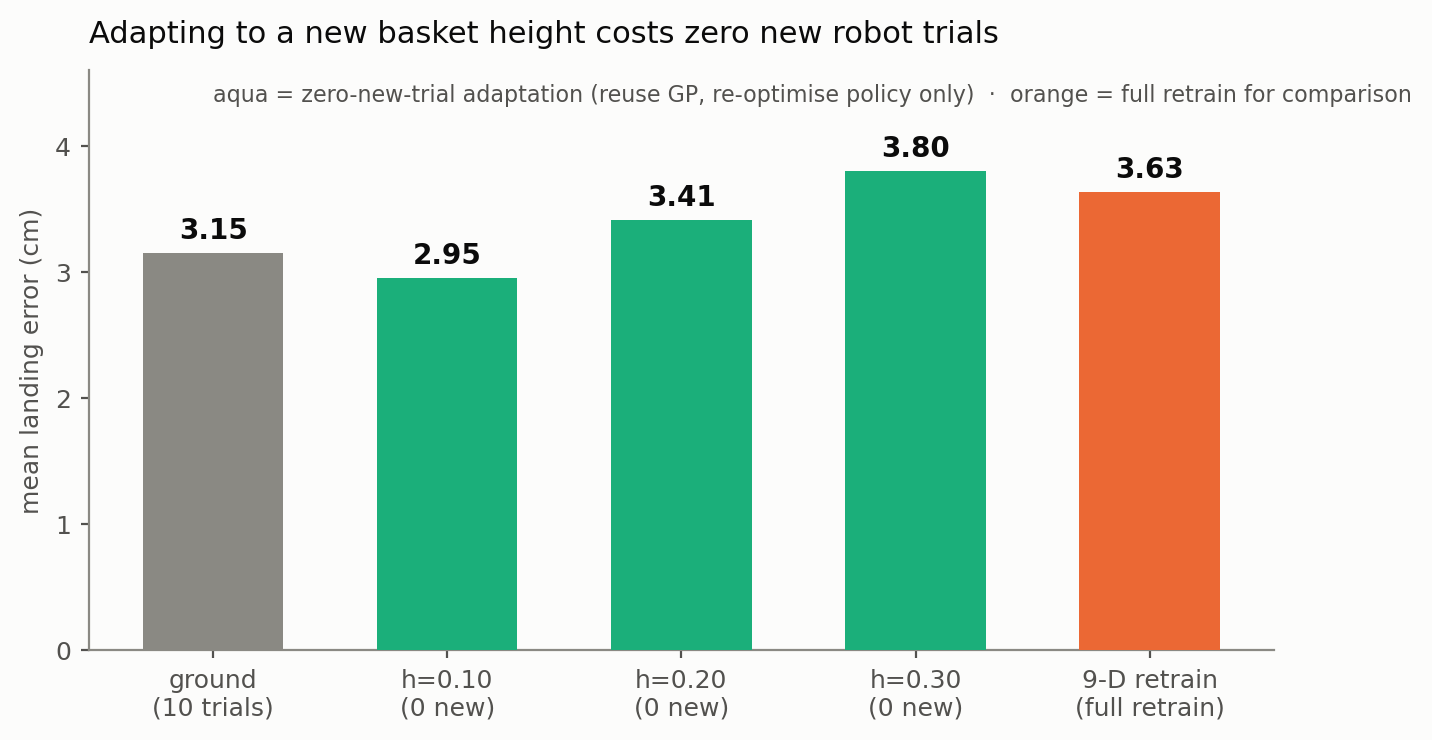
\includegraphics[width=0.9\linewidth]{../status_update/final_figures/fig_height_adaptation.png}
\caption{Zero-new-trials height adaptation: the trained GP is reused
verbatim and only the policy is re-optimized for each new height.}
\label{fig:height-adapt}
\end{figure}

\subsection{The overhead throw and an honest safety ceiling}
\label{sec:results-overhead}
For the Gen3's 9~Nm wrist actuators, achievable range under a fixed
low-release posture falls off monotonically with elevation angle, so a
distance-scoring pose search collapses to a near-horizontal push. Searching
the release \emph{state} directly under whole-trajectory feasibility
(Sec.~III-B/C) instead finds a genuine overhead throw: windup, whip, and
release at $\sim$1.1~m height. With whole-trajectory safety honestly
enforced -- including the post-release follow-through, which had no
feasibility check at all until this was added and was found to silently
command 3.2$\times$ torque and 1.9$\times$ joint-speed limits -- the
furthest this arm can safely throw is 0.83~m, just inside its own 0.87~m
kinematic reach (Fig.~\ref{fig:range-ceiling}). We report this as a
measured hardware capability boundary rather than a shortfall: with the
base fixed, this arm's contribution is precision and data efficiency of a
physically real release, not extended reach, which the higher-torque arms
in Sec.~\ref{sec:results-multiarm} (2.0--2.5~m/s release speed, 0.6--1.1~m
throws) demonstrate instead. On this final configuration: 3.15~cm mean
error, 100\% hits $<$10~cm, 30 unseen targets, 10 training trials, release
speed scaling correctly with target distance (1.16--1.49~m/s, not
saturated).

\begin{figure}[t]
\centering
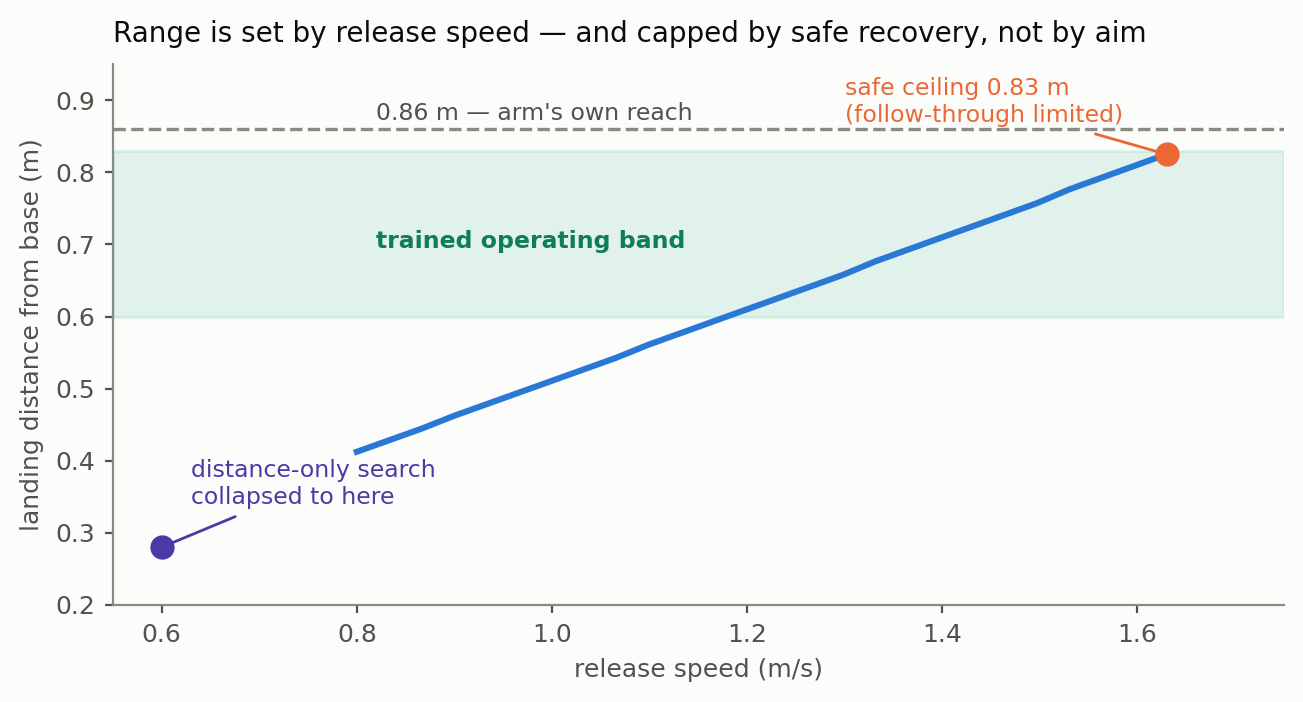
\includegraphics[width=0.9\linewidth]{../status_update/final_figures/fig_range_ceiling.png}
\caption{Measured safe-throw range ceiling (0.83~m) against the arm's own
kinematic reach (0.87~m) under whole-trajectory torque/velocity
feasibility.}
\label{fig:range-ceiling}
\end{figure}

\subsection{Feasibility-cascade ablation}
\label{sec:results-ablation}
To quantify what whole-trajectory feasibility checking
(Sec.~\ref{sec:method-feasibility}) buys over the release-instant-only
check used earlier in this project's own history, we re-ran the
release-pose search's exact candidate enumeration for the Gen3 and, for
comparison, a higher-torque arm (Franka Panda, 87/12~Nm vs.\ the Gen3's
39/9~Nm), recording for every candidate that clears the release-instant
criterion (static torque feasibility, kinematic windup bound, and torque
feasibility at the release instant alone) whether it also clears the full
whole-trajectory cascade. Table~\ref{tab:ablation} reports, per arm: the
number of release-instant-feasible candidates, the fraction of those that
whole-trajectory checking additionally rejects, the rejection breakdown by
stage (windup-path / throw-ramp / follow-through), and the best landing
distance found under each criterion.

\begin{table}[t]
\centering
\small
\caption{Release-instant-only vs.\ whole-trajectory feasibility checking,
same posture/direction grid, two arms.}
\label{tab:ablation}
\begin{tabular}{@{}lcc@{}}
\toprule
 & Gen3 & Panda \\
\midrule
Release-instant-feasible & 446{,}071 & 152{,}844 \\
Also full-traj.-feasible & 74{,}230 (16.6\%) & 152{,}844 (100\%) \\
Rej.\ windup-path & 242{,}725 (54.4\%) & 0 \\
Rej.\ throw-ramp & 66{,}706 (15.0\%) & 0 \\
Rej.\ follow-through & 62{,}410 (14.0\%) & 0 \\
Best range, instant-only & 1.03 m & 1.65 m \\
Best range, full check & 0.82 m & 1.65 m \\
\bottomrule
\end{tabular}
\end{table}

On the Gen3, whole-trajectory checking rejects \textbf{83.4\%} of candidates
that a release-instant-only check would have accepted as feasible.
Contrary to our own expectation going in -- that follow-through, the check
added latest to this pipeline's history, would dominate -- the single
largest rejector is actually the \emph{windup-path} check (54.4\% of
release-instant-feasible candidates, vs.\ 15.0\% for throw-ramp and 14.0\%
for follow-through; percentages are of the release-instant-feasible set and
overlap, since a candidate can fail more than one stage and we report the
first failure in cascade order). This means most of the false accepts from
a weaker check are postures whose neutral$\to$windup swing passes through
an intermediate gravity configuration worse than either endpoint -- a
failure mode invisible to any check that only looks at the release state,
regardless of how sophisticated that release-state check is. Consistent
with the safety-ceiling finding in Sec.~\ref{sec:results-overhead}, the
release-instant-only search's best candidate (1.03~m) overstates the
actually-recoverable range by 25\% relative to the full-trajectory result
(0.82~m, matching the production search's shipped 0.824~m table entry to
three decimal places) -- i.e., without whole-trajectory checking, this
pipeline would have shipped a release the arm cannot actually recover
from.

On the Panda, whole-trajectory checking rejects \textbf{0} of the 152{,}844
release-instant-feasible candidates -- every one already clears the full
cascade, and the best candidate under either criterion is identical (bit-
for-bit, since it is the same argmax). This is the clean version of the
story the Gen3 numbers tell obliquely: whole-trajectory feasibility
checking only \emph{matters} when torque is close to the binding
constraint. The Panda's 87/12~Nm torque budget (vs.\ the Gen3's 39/9~Nm)
leaves enough headroom that release-instant feasibility already implies
whole-trajectory feasibility for every candidate this search considered.
This is also, we suspect, why the original paper's fixed-pose design never
needed this check: on a Panda, the gap this contribution closes is empty.

\subsection{Computational cost}
\label{sec:results-cost}
A full training run for the Gen3 overhead-throw configuration (10 trials,
5 exploration, $N_{opt}=1500$ policy-optimization steps per trial,
reusing a pre-computed pose table) took 17~min~44~s wall-clock on a single
CPU core (no GPU; consistent with this project's earlier finding that GPU
is not faster for this workload's tensor sizes), peak memory 1.11~GB.
The one-time release-pose search itself (Sec.~\ref{sec:method-search},
\texttt{find\_throw\_pose.py --mode overhead}, $\sim\!9\times10^4$ posture
candidates before pruning) took 28~min~27~s wall-clock on the same
machine, single CPU core. Both are one-time-per-arm costs, not per-trial or per-target
costs: the pose table is reused across all training seeds and evaluation
targets for a given arm/floor geometry, and re-optimizing a policy for a
new target height (Sec.~\ref{sec:results-height}) reuses the trained GP and
takes a small fraction of a full training run's time.

\subsection{Real hardware bring-up}
\label{sec:results-hw}
Table~\ref{tab:hw-status} summarizes what has been validated live on the
real Gen3 to date. Bring-up surfaced and fixed several real,
previously-invisible issues: a joint-angle reporting convention in which
every joint (including limited ones) is reported on $[0^\circ,360^\circ)$,
requiring different homing logic for continuous vs.\ limited joints;
gripper release latency, measured at $67.9\pm6.4$~ms over 1~kHz UDP
feedback, which at the 1.498~m/s release speed used in the overhead throw
corresponds to a 10.2~cm undershoot if uncompensated -- 3.5$\times$ the
entire simulation accuracy budget -- and is compensated as a wall-clock
lead time in the executor; a control-loop rate correction (the streaming
interface's documented ceiling is 40~Hz, not the 1~kHz figure that belongs
to an unused low-level servoing path); and measured open-loop position
drift during the throw of 0.0171~rad at release, which back-converts to
$\approx$1.0~cm of landing error, inside the simulation's 2.89~cm accuracy
budget -- indicating open-loop joint-speed streaming is a viable control
strategy for this throw. \texttt{connect}, \texttt{home}, \texttt{gripper},
and an empty-gripper throw have since all been executed and accepted live
at all four rehearsal speed scales (0.15/0.30/0.60/1.00), and the
0.500~m/s Cartesian speed ceiling (\texttt{twist\_linear}) initially flagged
as an open risk was confirmed not to apply in joint-speed streaming mode --
both by a direct firmware read (that field is unset for the streaming mode
this throw uses) and by the empty-gripper full-speed rehearsal completing
clean with no fault. Gripper release latency, re-measured with a real ball
loaded over 15 trials, is $73.2\pm10.3$~ms -- statistically indistinguishable
from the static/unloaded figure above, which validates the onset
measurement specifically, though not yet its contribution to a real landing
error.

\textbf{A gripper release command is silently dropped while joint speeds
are streaming.} Several real ball throws were executed at escalating speed
scales before this was found: \texttt{SendGripperCommand} is accepted and
acknowledged by the SDK but produces zero physical motion for as long as
\texttt{SendJointSpeedsCommand} is being actively streamed on the same
session -- reproduced with an isolated test, arm not even moving, zero
velocities streamed, and with no exception or elevated command latency to
flag it, which is why several earlier throws had no way to distinguish a
genuine open-gripper release from the ball simply leaving the hand under
arm deceleration. A second, gripper-dedicated session is not a fix: only
the session already in control of the arm may issue any command, gripper
included, and a second session is rejected outright rather than silently
ignored. The fix is a 200~ms pause in the \emph{same} session's joint-speed
stream immediately after the release-time open command, coasting the arm at
its release-instant velocity rather than the planned follow-through
deceleration during the gap (checked against joint limits at the trained
release state: worst-case margin 76.4$^\circ$ at a 300~ms pause, so 200~ms
is conservative). Verified 2-for-2 on the real arm with an empty gripper
(fully open, 0.87\% closed, both runs, no fault); not yet re-verified with a
ball loaded.

\textbf{The release model, shared by simulation and hardware, has always
assumed a zero-length end effector.} The release-pose solver
(Sec.~\ref{sec:method-search}) and the simulated ball's attachment point
both use the bare wrist flange with no tool offset -- consistent between
the two, but neither has ever accounted for the real Robotiq 2F-85
gripper's reach. The offset is not a guess: reading the arm's own tool
configuration (\texttt{GetToolConfiguration}, read-only) returns a
0.12~m offset along the tool $z$-axis and a 0.831~kg tool mass, matching a
real 2F-85 and evidently configured deliberately on this arm rather than
left at a manufacturer default. At the trained release state
($\omega\approx3.25$~rad/s), the resulting velocity correction
$v_{true} = v_{flange} + \omega\times r_{offset}$ works out to 0.39~m/s --
26\% of the 1.498~m/s release speed used throughout this paper's hardware
results -- and a 12.0~cm position offset at release: an order of magnitude
larger than every other hardware error source in
Fig.~\ref{fig:error-budget} combined. The fix is to fold
$r_{offset} = R(q)\cdot[0,0,0.12]$ into the shared release solver's
position and velocity outputs, re-run the release-pose search
(Sec.~\ref{sec:method-search}), and re-verify feasibility before any
further ball throw is treated as a data point. This is scoped but not yet
implemented, and is the reason Table~\ref{tab:hw-results} remains empty.

\textbf{Landing measurement.} Independent of the release-model fix, the
stereo-infrared landing-measurement pipeline (Sec.~\ref{sec:setup}) has
been run against real captured frames for the first time: on a real throw
capture, 119 of 130 frames were successfully paired across both IR
streams, and the resulting triangulated 3D track forms a smooth,
continuous arc on visual inspection, matching the sub-millimeter accuracy
this pipeline reached on synthetic-only validation before any real frame
existed. The camera-to-base extrinsic needed to express that track in the
arm's own frame, however, is still the earlier, marginal-quality
laptop-rig calibration rather than the final overhead mount -- so every
real-frame result to date is a relative, pixel-space verification, not yet
an absolute landing-position measurement.

\begin{table}[t]
\centering
\small
\caption{Real Kinova Gen3 hardware bring-up status.}
\label{tab:hw-status}
\begin{tabular}{@{}p{4.6cm}c@{}}
\toprule
Stage & Status \\
\midrule
Read-only state (joints, gripper) & live \\
Gripper actuation & live \\
Full-speed joint-vel.\ streaming (all scales) & live \\
Gripper latency compensation (loaded) & done \\
Gripper-release-during-streaming bug & fixed \\
Open-loop drift budget & in budget \\
Loaded throw (ball in gripper) & \textcolor{orange}{\textbf{done, not valid}} \\
Release TCP-offset correction & \textcolor{red}{\textbf{pending}} \\
Real landing measurement & \textcolor{red}{\textbf{pending}} \\
\bottomrule
\end{tabular}
\end{table}

\begin{figure}[t]
\centering
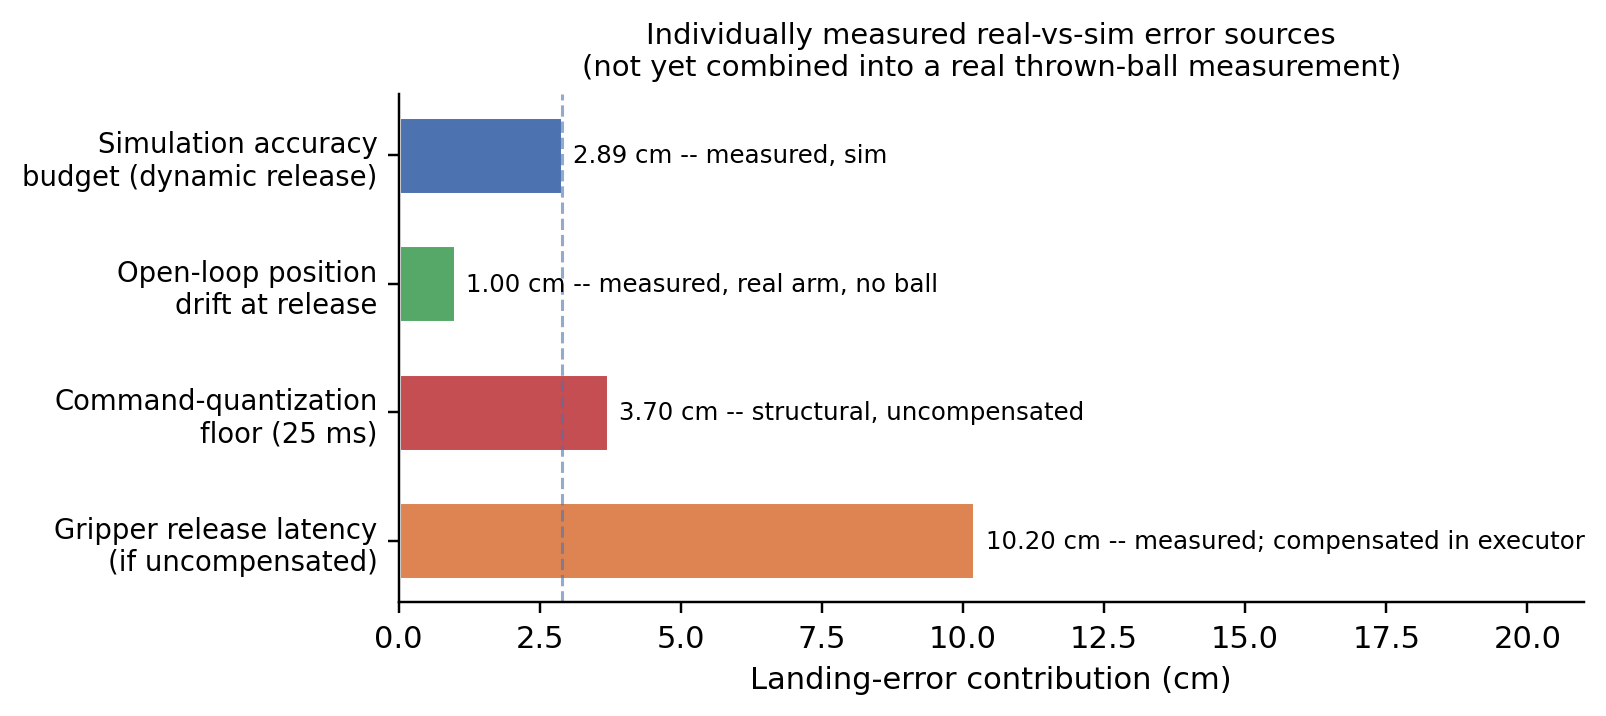
\includegraphics[width=\linewidth]{figs/error_budget_waterfall.png}
\caption{Individually measured sim-vs-real error sources found during
bring-up, plotted against the simulation accuracy budget. These are
separately measured quantities, not yet combined into one real
thrown-ball measurement -- some (gripper latency) are already compensated
in the executor; others (command quantization) are not.}
\label{fig:error-budget}
\end{figure}

Fig.~\ref{fig:error-budget} places these measurements against the
simulation accuracy budget. The gripper-latency term, uncompensated, would
dominate every other error source combined; compensated, its residual
contribution has not yet been isolated by a real throw. The
command-quantization floor (25~ms command interval, $\approx$3.7~cm) is
the one term identified but not yet addressed, and is a candidate
explanation if real accuracy comes in above the simulation budget even
after a loaded throw succeeds. The end-effector offset described above was
found after this figure was generated and is not plotted in it; at 12~cm
it would dwarf every bar shown, so the figure should be read as the error
budget \emph{given} a correctly modeled release point, not the full picture
as of this draft.

\hwtodo{Real thrown-ball results go here once: (i) the end-effector-offset
correction above is folded into the shared release solver and the
release-pose search re-run, (ii) a loaded throw re-verifies the
gripper-release-pause fix, (iii) the camera is remounted on its final
overhead rig and the camera-to-base extrinsic re-measured, and (iv) 10 real
MC-PILOT calibration trials plus evaluation on 10--15 held-out real targets
are run through the corrected pipeline. Table~\ref{tab:hw-results} is the
template for that result -- fill in rows, do not fabricate them.}

\begin{table}[t]
\centering
\small
\caption{\hwtodo{Real Gen3 throwing eval.\ (template, N/A until real
trials run).}}
\label{tab:hw-results}
\begin{tabular}{@{}cccc@{}}
\toprule
Target \# & Speed (m/s) & Error (cm) & Hit? \\
\midrule
\hwdash & \hwdash & \hwdash & \hwdash \\
\bottomrule
\end{tabular}
\end{table}

\section{Discussion and Limitations}

\textbf{No valid real landing has been measured yet.} Every accuracy number
in Sec.~\ref{sec:results-baseline}--\ref{sec:results-overhead} is a
simulation result. Sec.~\ref{sec:results-hw} shows every non-destructive
stage of the real pipeline validated live, and several real ball throws
executed, but a 12~cm-scale release-model error was found after those
throws and is not yet corrected, so none of them is a usable data point.
This, not hardware access, is now the central open item of the paper, and
is why Table~\ref{tab:hw-results} is presented empty rather than omitted.

\textbf{The landing-measurement pipeline's absolute accuracy is
unverified.} The stereo-infrared triangulation and ballistic fit
(Sec.~\ref{sec:setup}) have been run on real captured frames and produce a
visually clean 3D track, but the camera-to-base extrinsic used to express
that track in the arm's own frame is a superseded, marginal-quality
calibration -- so no real landing number in this paper, once one exists,
should be read as more accurate than that extrinsic allows.

\textbf{Delay is a point estimate, not a fitted distribution.} The
original paper models gripper-open delay as a learned probability
distribution, estimated by Bayesian optimization and propagated
stochastically through policy optimization. Our Gen3 work instead directly
measures a single latency value at high rate and compensates it as a fixed
lead time. This is more directly grounded (measured on the actual gripper
hardware, not inferred from throw outcomes) but less general -- it does not
capture delay \emph{variance}, which the original approach does. A
reviewer familiar with~\cite{turcato2025mcpilot} should expect this
comparison and we state it plainly rather than let it surface as a
surprise.

\textbf{Object generalization is simulation-only here.} The original paper
tests five real objects with real material and shape variety (rubber ball,
tennis ball, cube, cylinder, hammer); our object-generalization result
(Sec.~\ref{sec:results-multiarm}) sweeps payload mass and size in
simulation only.

\textbf{Multi-arm generalization is simulation-only.} The four-manipulator
result has not been run on a second piece of real hardware; only the Gen3
has a real bring-up in progress.

\textbf{Reproducibility.} The release-pose search solver, whole-trajectory
feasibility checker, multi-arm evaluation scripts, and trained GP/policy
checkpoints for every simulation result in this paper will be released
publicly on acceptance; the anonymized code is available to reviewers on
request through the venue's mechanism for anonymous artifact access.

\section{Conclusion}

We extended MC-PILOT along the axis its fixed-release-pose design leaves
unaddressed: making the release configuration itself part of what is
searched, under real torque and whole-trajectory feasibility constraints,
which is what makes a lower-torque 7-DOF arm throwable under this framework
at all. Along the way, a reliability audit corrected a single-seed
convergence claim, a continuous height-generalized policy went beyond the
original paper's discrete demonstration, and a quantified drag-regime
crossover identified exactly when the learned model earns its cost over an
analytical baseline. Every non-destructive stage of the resulting pipeline
has been validated on a real Kinova Gen3, and bring-up itself surfaced two
further findings worth reporting on their own terms: a gripper-release
command silently dropped mid-stream, now fixed, and a shared sim/hardware
release model that has always assumed a zero-length end effector, now
quantified but not yet corrected. \hwtodo{Closing sentence to be rewritten
once real throwing results land through the corrected pipeline: state the
headline real-hardware number here, and whether it matches, exceeds, or
falls short of the simulation-predicted 2.89~cm accuracy budget from
Sec.~\ref{sec:results-hw}.}

% Acknowledgments intentionally omitted for double-anonymous review.
% Re-add before camera-ready, including any required generative-AI
% disclosure per the current ICRA policy.

\begin{thebibliography}{9}

\bibitem{turcato2025mcpilot}
N.~Turcato, G.~Giacomuzzo, M.~Terrean, D.~Allegro, R.~Carli, A.~Dalla
Libera, ``Data efficient Robotic Object Throwing with Model-Based
Reinforcement Learning,'' arXiv:2502.05595, 2025.

\bibitem{amadio2022mcpilco}
F.~Amadio, A.~Dalla Libera, D.~Nikovski, R.~Carli, D.~Romeres,
``Model-based policy search via Monte Carlo gradient estimation with real
system applications,'' \emph{IEEE Transactions on Robotics}, vol.~38,
no.~6, pp.~3879--3898, 2022.

\bibitem{turcato2023codit}
N.~Turcato, A.~Dalla Libera, G.~Giacomuzzo, R.~Carli, ``Teaching a robot to
toss arbitrary objects with model-based reinforcement learning,'' in
\emph{2023 9th International Conference on Control, Decision and
Information Technologies (CoDIT)}, 2023, pp.~1126--1131.

\bibitem{zeng2020tossingbot}
A.~Zeng, S.~Song, J.~Lee, A.~Rodriguez, T.~Funkhouser, ``TossingBot:
Learning to throw arbitrary objects with residual physics,'' \emph{IEEE
Transactions on Robotics}, vol.~36, no.~4, pp.~1307--1319, 2020.

\bibitem{coumans2021pybullet}
E.~Coumans and Y.~Bai, ``PyBullet, a Python module for physics simulation
for games, robotics and machine learning,'' 2016--2021.
\url{http://pybullet.org}

\end{thebibliography}

\end{document}
